\documentclass{standalone}
\usepackage{tikz}
\usepackage{pgfplots}
\begin{document}
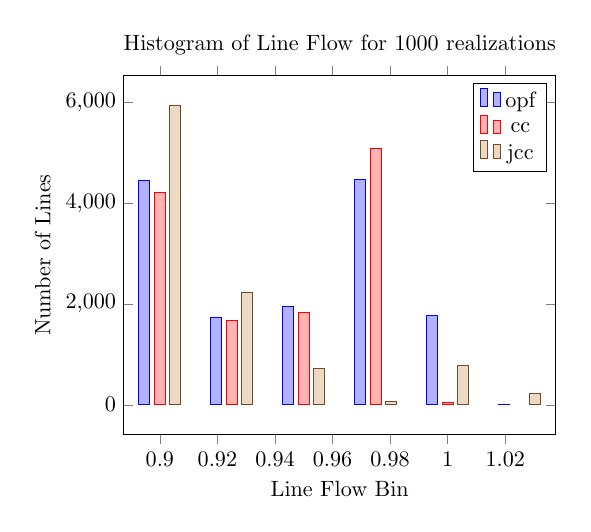
\begin{tikzpicture}[scale=.8]
\begin{axis}[title=Histogram of Line Flow for 1000 realizations, 
    xlabel=Line Flow Bin, 
    ylabel=Number of Lines,
x tick label style={
/pgf/number format/1000 sep=},
  ybar, bar width=5pt ,
  enlargelimits=0.1]
\addplot coordinates { ( 0.9,4450)  ( 0.925,1729)  ( 0.95,1949)  ( 0.975,4471)  ( 1,1770)  ( 1.025,3) };
\addplot coordinates { ( 0.9,4219)  ( 0.925,1678)  ( 0.95,1834)  ( 0.975,5077)  ( 1,53) };
\addplot coordinates { ( 0.9,5931)  ( 0.925,2218)  ( 0.95,711)  ( 0.975,70)  ( 1,784)  ( 1.025,221) };
\legend{opf,cc,jcc}
\end{axis}
\end{tikzpicture}
\end{document}
